\documentclass[fleqn, a4paper]{report}

%% Language and font and usefull packages
\usepackage[english]{babel}
\usepackage[utf8x]{inputenc}
\usepackage{booktabs}
\usepackage{tabu}
\usepackage[T1]{fontenc}
\usepackage{bm}
\usepackage{setspace}
\usepackage{amsmath}
\usepackage{graphicx}
\usepackage{titlepic}
\usepackage{booktabs} % For prettier tables
\usepackage[colorinlistoftodos]{todonotes}
\usepackage[colorlinks=true, allcolors=blue]{hyperref}
\usepackage[a4paper,top=3cm,bottom=3cm,left=1.5cm,right=1.5cm,marginparwidth=1.75cm]{geometry}

%\graphicspath{ {./images} }
\title{Assignment 2 - Simulation Experiment}
\author{
Theodoros Ladas - s2124289 
\footnote{University of Edinburgh s2124289@ed.ac.uk}
}
\titlepic{
\includegraphics[width=12.528cm,height=3cm]{./images/edinburgh.png}} 
\date{\parbox{\linewidth}{\centering%
  January 10, 2021\endgraf\bigskip
  Coordinator: Miguel de Carvalho\endgraf\medskip
  Dept.\ of Mathematics \endgraf
  University of Edinburgh}}


%\onehalfspacing
\begin{document}
\maketitle

\section*{1. Experiment}







\subsection*{1.1. Data generating processes}

\subsection*{1.2. KDE vs Histogram}


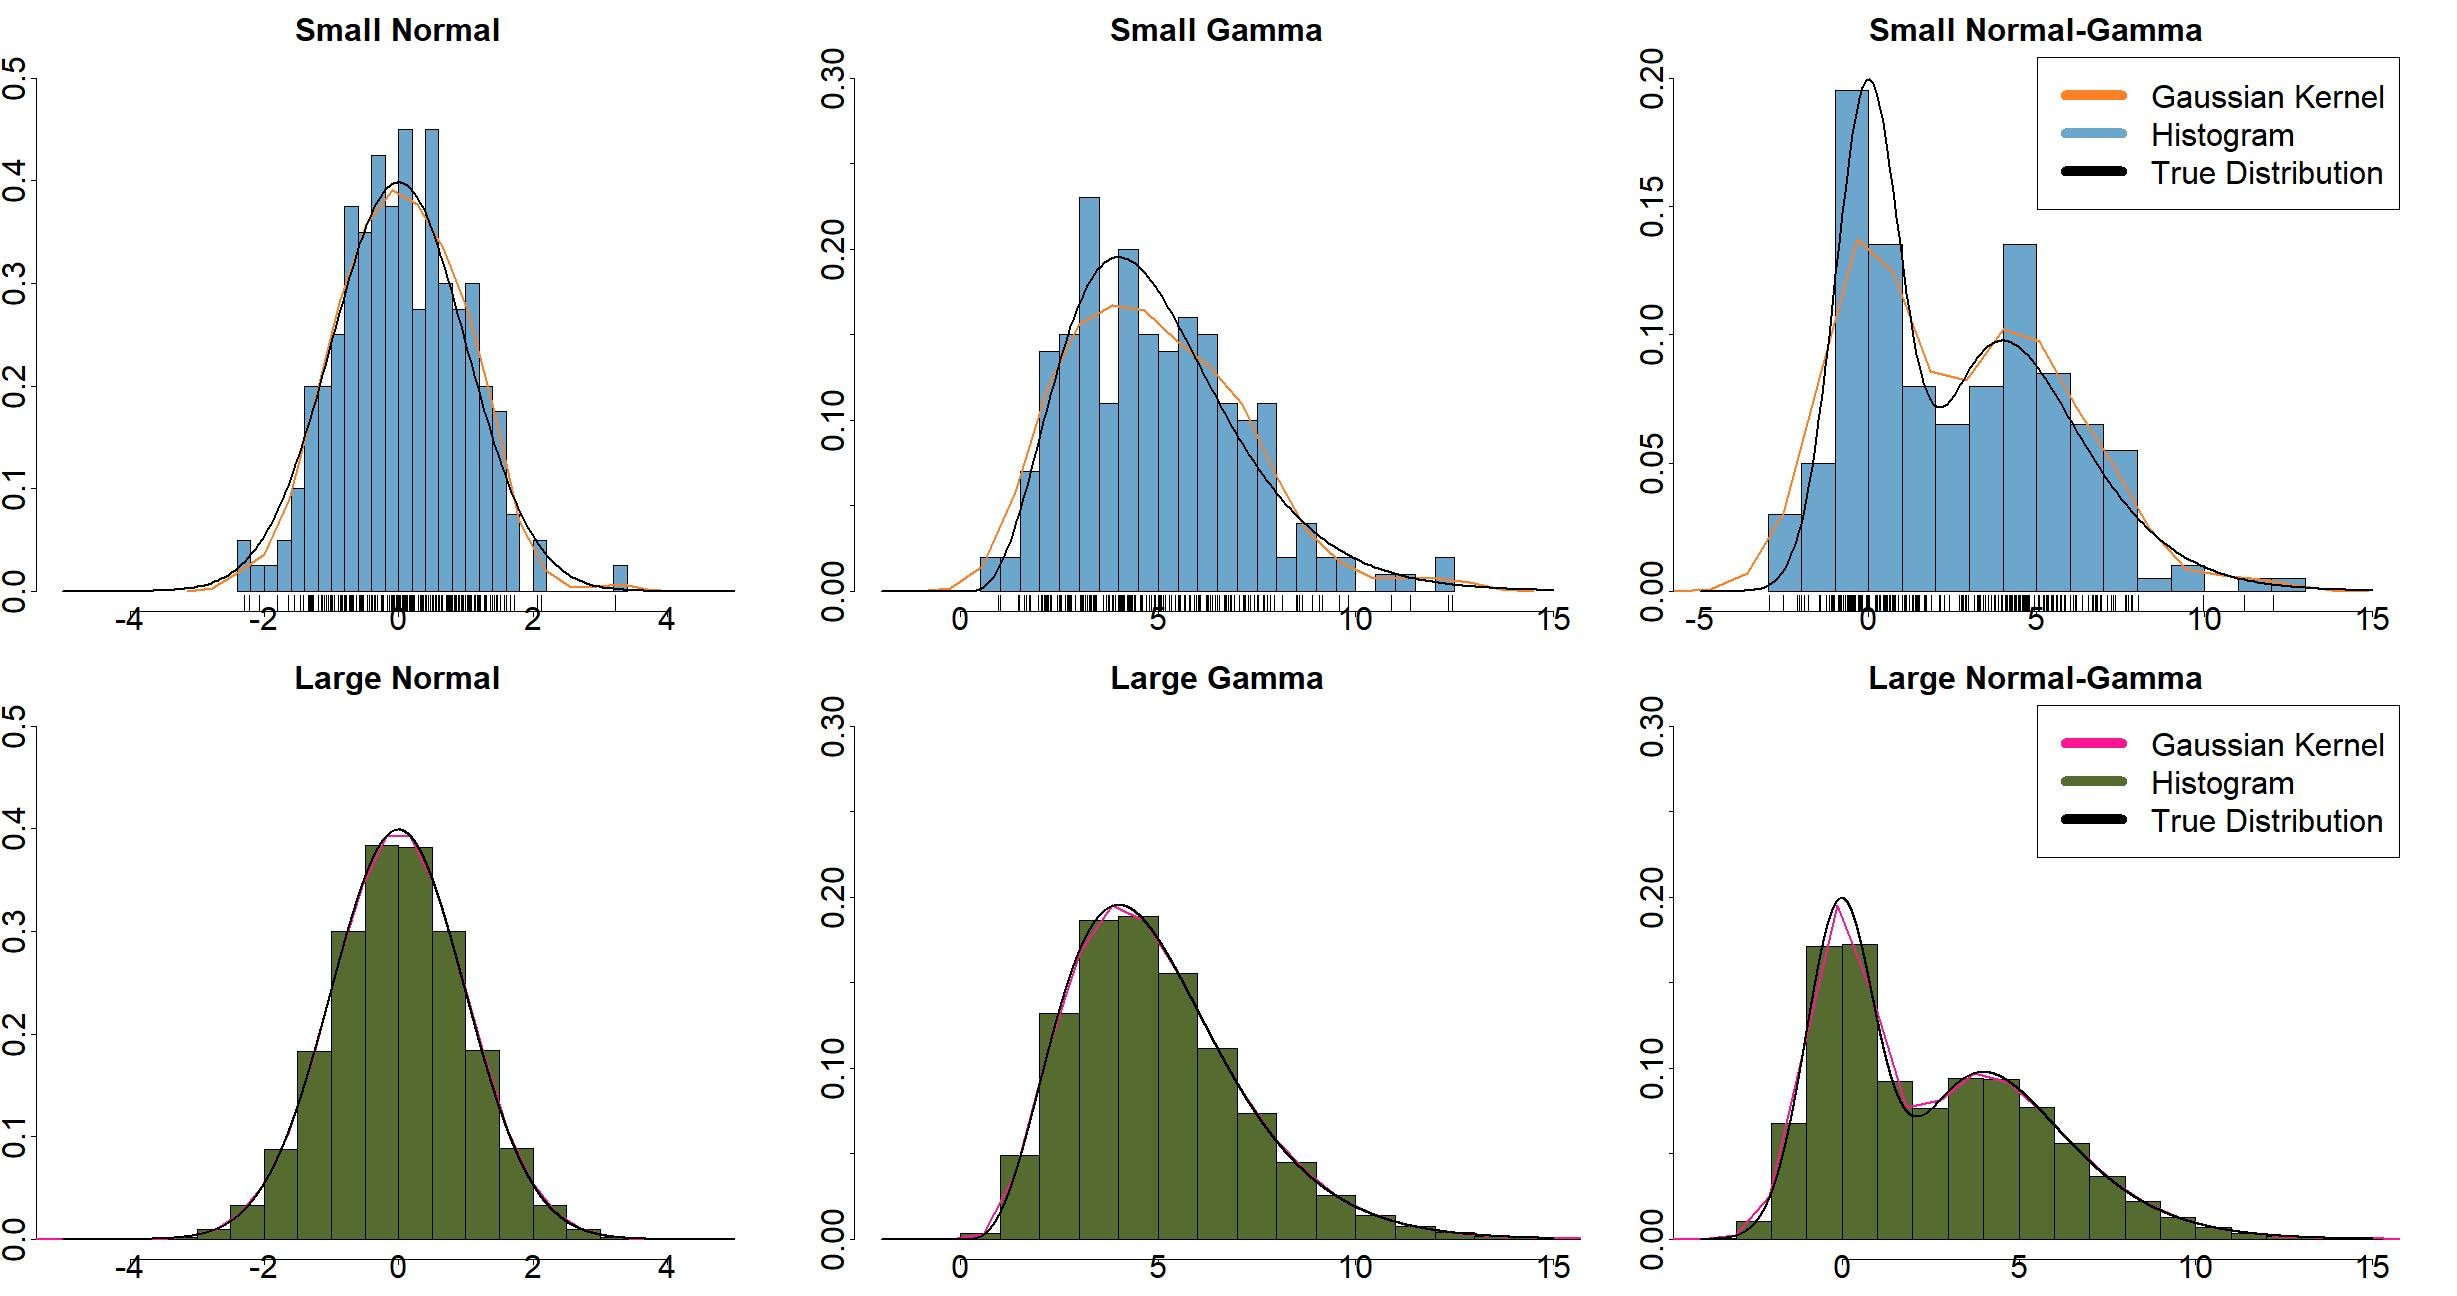
\includegraphics[width=0.6\textwidth]{./images/hist_vs_GKDE.jpg}



\section*{2. Monte Carlo}


\begin{tabular}{|l|lll|}
\hline
n    & Normal & Gamma & Mixture \\ \hline
250  & 8.612  & 4.092 & 0.092   \\
500  & 8.013  & 3.994 & 0.101   \\
1000 & 8.095  & 3.879 & 0.117   \\ \hline
\end{tabular}



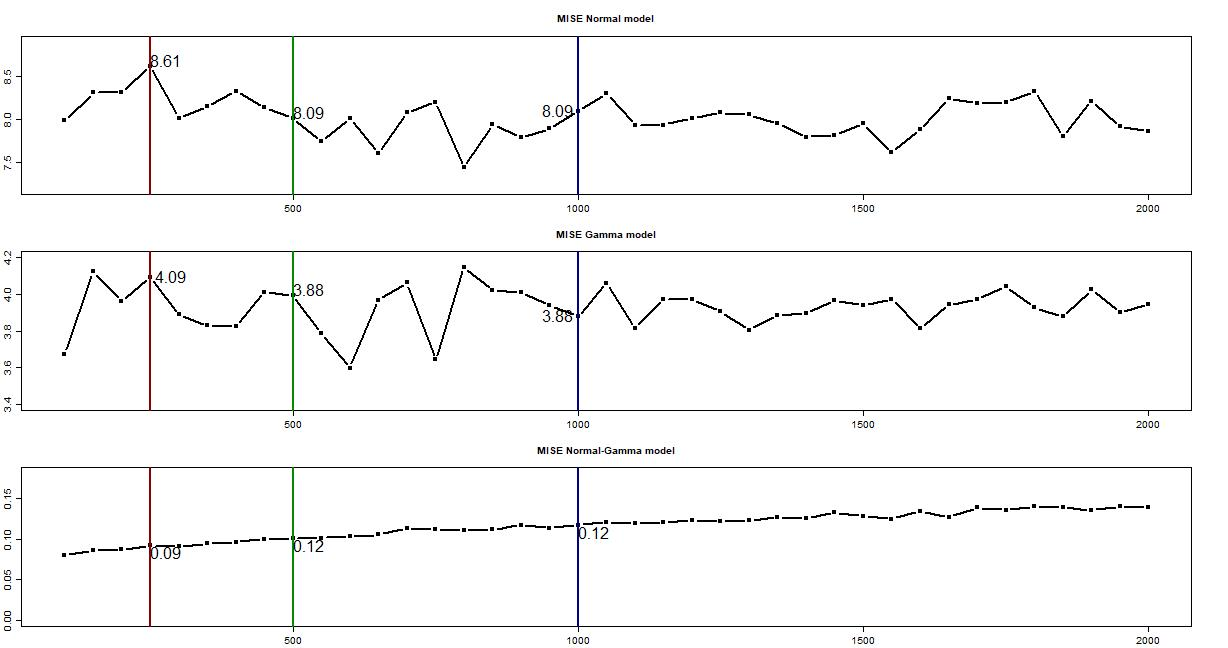
\includegraphics[width=1\textwidth]{./images/MISE error.jpg}



\section*{3. Conclusion}

\bibliographystyle{plain}
\bibliography{assignment_2_references.bib}

\end{document}
























